
%
%  $Description: Application Scheduling in CloudSim$ 
%
%  $Author: Pradeeban $
%  $Date: 2013/11/20 17:04:59 $
%  $Revision: 1.4 $
%

\documentclass[times, 10pt,twocolumn]{article} 
\usepackage{cloudsim}
\usepackage{times}
\usepackage{moreverb}
\usepackage{amsmath}
\usepackage{graphicx}     % to include images
\usepackage[utf8]{inputenc}
\usepackage[T1]{fontenc}

%\documentstyle[times,art10,twocolumn,cloudsim]{article}

%------------------------------------------------------------------------- 
\pagestyle{empty}

%------------------------------------------------------------------------- 
\begin{document}

\title{Application Scheduling in CloudSim}

\author{Pradeeban Kathiravelu\\
KTH Royal Institute of Technology, Stockholm, Sweden.\\ kpr@kth.se\\
}

\maketitle
\thispagestyle{empty}

\begin{abstract}
   Cloud computing involves a  hierarchy of dispersed with distributed shared resources, such as processor, memory, and bandwidth. Many of the user-submitted tasks require a considerable amount of resources to be allocated exclusively for them for a successful operation. Jobs should be scheduled in a felicitous manner for an efficient execution. Application scheduling algorithms are implemented to fairly schedule the jobs of the users to the available resources. Prior to test the scheduling algorithms in the real cloud environment, they are often tested on a simulation environment such as CloudSim or EmuSim. This paper looks into the three families of application scheduling algorithms --- strict matchmaking-based, utility-driven, and QoS-driven algorithms, and evaluates the algorithms to find their performance and scheduling efficiency. 
\end{abstract}


\textbf{Categories and Subject Descriptors}\\
D.2.8 \textbf{[Software Engineering]}: Operating Systems --- scheduling\\
D.2.8 \textbf{[Software Engineering]}: Metrics --- performance measures\\
\textbf{General Terms}\\
Simulation\\
\textbf{Keywords} ---  Application Scheduling, Strict Matchmaking-based algorithms, Utility-driven algorithms, QoS-driven algorithms, Cloud Simulation, VM (Virtual Machine).

%------------------------------------------------------------------------- 
\Section{Introduction}

Application scheduling plays a major role in a system that has resources distributed and shared among the users. Fair scheduling of the resources is mandatory for a successful execution of the system. With the ever increasing complexity of the cloud environments such as the heterogeneity and geographic dispersion of the cloud resources, as well as the users submitting the applications from different geographic locations, scheduling the applications has become a harder task to accomplish, making it a promising research field. Scheduling algorithms are developed to find a resource for any given job that fulfils the job requirements. Three families of algorithms are developed to address this, naming, strict matchmaking-based algorithms, utility-driven algorithms, and QoS-driven algorithms.

Strict matchmaking-based scheduling algorithms perform well for certain tasks as they focus on total fulfilment of the specified requirement of the job which is specified as an objective function. Utility is a measure of user's satisfaction, which could be expressed as a composite of objective functions that the scheduler aims to optimize. While these algorithms focus to optimize a specific objective function, they do not consider partial requirements satisfaction, where the requirements from the users are satisfied partially based on the utility value given to each of the user requirements\cite{resumo}. Hence, these algorithms do not satisfy the varying scheduling needs of the users in a real world cloud environment.

Utility-driven and QoS-driven algorithms focus to mitigate the shortcomings of the strict matchmaking-based algorithms. Utility-driven algorithms consider the partial requirement satisfaction, where the application requirements and the objective functions are considered and satisfied partially by the algorithm based on the importance of the requirement to the user. QoS-driven algorithms ensure the quality of service measures, in addition to the existing algorithms. 

This research targets to evaluate the user satisfaction of different application scheduling algorithms. Due to the complicated nature of the cloud environments, Cloud Simulation tools are used in the early phases of research, development, and testing of the applications, opposed to implementing and testing on the real cloud environments. During this research, the scheduling algorithms will be incorporated and evaluated on CloudSim\cite{cloudsim}, an open source cloud simulation tool implemented using Java. 

In the upcoming sections, we will further analyse the application scheduling algorithms and how they behave in cloud environments, by studying their behaviour using CloudSim. We will continue to discuss the preliminary background information on application scheduling algorithms, in section II. Section III discusses the design and implementation where we will analyse the design and implementation of the application scheduling algorithm, and how CloudSim is customized and extended to incorporate the application scheduling algorithms. Section IV consists of evaluation which is a detailed discussion on the experimental studies of the scheduling algorithms, the efficiencies of the scheduling algorithms on CloudSim, and the results produced by the studies. Finally, section V will drive us to the conclusion of this research.
%------------------------------------------------------------------------- 
\Section{Preliminaries}

%------------------------------------------------------------------------- 
\SubSection{Strict Matchmaking-based Algorithms}
Strict matchmaking-based algorithms focus on a specific objective function and attempt to optimize the scheduling accordingly. First-come first-served (FCFS), round-robin (RR), matchmaking algorithm, minimum execution time (MET), minimum completion time, (MCT), min-min, and max-min\cite{heuristics} are notable examples of strict matchmaking-based algorithms. 

FCFS schedules the tasks according to the order they arrived. Hence a task or a user that arrived first will be considered before the one that arrived later. RR is on the other hand allocates a time slot for each of the tasks or users. A task will be assigned when its slot is reached, and executed as long as its slot lasts. Once the slot finishes, the slot will be assigned to the next in the round and the algorithm moves on serving everyone in a time-shared fashion. In a FCFS system, if a bigger task comes first, the smaller tasks that arrive later will have to wait for a long time, or even starve to death. In a RR system, a bigger task will have to wait for a long time to complete as time is shared among all the tasks by allocating them a time slot regardless of the submission time or the order of submission. This may lead to a bigger task being timed out.

Matchmaking algorithm finds a resource that matches the specification of an application. The application specification could be the operating system or the computer architecture. In the heterogeneous cloud environment, overly constrained applications may fail to find the resource with the specified requirements in a given time limit. Job scheduling success ratio could be used as a measure to evaluate the matchmaking algorithm. 

%------------------------------------------------------------------------- 
\SubSection{Utility-driven Algorithms}
Matchmaking-based algorithm schedules the application to satisfy the specified objective function. In a market-oriented cloud environment, the objective function is often a composite of variable requirements such as the execution time as well as the cost and the user priorities. Users have different priorities over these different criteria. A few of these criteria may have a lower priority such that they could be ignored in favour of a parameter that is of a higher priority to the user. This is defined as Partial requirement satisfaction. The utility value of the objective functions could be in the range from 0 to 1, where 1 indicates the highest priority and negligible priorities approach 0 value. Utility-driven algorithms consider the user- or system- defined utility functions and the user determines the utility-values for these functions. Since these algorithms could be designed to fit specific business scenarios, utility-driven algorithms are an interesting research domain.

%------------------------------------------------------------------------- 
\SubSection{QoS-driven Algorithms}
Some tasks are time constrained and their time-to-deliver is crucial for the success of the application. Such system or user critical tasks should be given higher priority to ensure the effective execution of the application. QoS priority-based scheduling algorithms categorize the tasks according to their priority as high and low. QoS Guided Weighted Mean Time-min (QGWMT) and QoS Guided Weighted Mean Time Min-Min Max-Min Selective (QGWMTMMS) are two such QoS-driven algorithms\cite{qosgrid}. 

%------------------------------------------------------------------------- 
\SubSection{Evaluation Criteria}
Performance and scheduling efficiency of these algorithms are measured by criteria such as job scheduling success ratio, average user utility, mean user submission time, mean execution time, mean completion time, average resource utilization, and Sufferage. Evaluation criteria for the scheduling algorithms are developed based on the objective functions, as they measure the effectiveness of the algorithms in a straight-forward manner. As strict matchmaking-based often focuses on a single objective function, they perform excellently for those specific objective functions. Mean execution time is the average of the time that each task spent executing. Minimum Execution Time (MET) algorithm targets a minimal execution time for the tasks. Mean submission time is the average of the time taken to submit the cloudlet for scheduling. Completion time is a total of the submission time and execution time, as execution follows submission. Minimum Completion Time
 (MCT) algorithm targets a minimal completion time of the scheduled tasks.

Job scheduling success ratio is how many of the submitted tasks were successfully scheduled in the considered time frame without timed out. Sufferage is the difference between the best and the second best completion time for the given task\cite{sufferage}. Minimal mean sufferage could be an objective function in a strict matchmaking-based algorithm.


%------------------------------------------------------------------------- 
\Section{Design and Implementation}
Researches involving complicated systems are often done on the simulation environments that try to mimic the real work environments as the access to the real environment is limited. Simulations empower the researchers with an effective and quicker way to test the prototype development of their research. As cloud computing environments consist of data centers and applications distributed on a planetary-scale, cloud simulations are used in evaluating the algorithms and strategies that are under research and development. CloudSim, EmuSim\cite{emusim}, and DCSim\cite{dcsim} are some of the mostly used cloud simulation environments. Simgrid\cite{simgrid} is a toolkit for the simulation of application scheduling. OverSim\cite{oversim} and PeerSim\cite{peersim} are simulation toolkits for overlay networks and peer-to-peer networks respectively. Among these simulation environments, CloudSim is frequently used by the researchers, because of its extensibility and portability. 

\SubSection{CloudSim}
Originally developed as GridSim, a Grid Simulation tool, CloudSim was later extended as a Cloud Simulation environment having GridSim as a major building block\cite{cloudgridsim}. Its modular architecture facilitates customizations. Hence it is extended by many researchers into different simulation tools such as CloudAnalyst\cite{cloudanalyst}, GreenCloud\cite{greencloud}, and NetworkCloudSim\cite{ncloudsim}. Developed in Java, CloudSim is portable. It could easily be incorporated with the scheduling algorithms with different parameters since its source code is open. For these obvious advantages, CloudSim was picked as the platform to evaluate the scheduling algorithms, and built from the source code using maven, incorporating the changes. CloudSim comes with examples to provide a quick start for using CloudSim for the simulations.

\SubSection{Architecture}
Components and characteristics of a basic cloud environment is depicted using the class hierarchy of CloudSim. The characteristics of the components of the cloud are depicted by the parameters and variables of the classes. CPU unit is defined by $Pe$ (Processing Element) in terms of millions of instructions per second (MIPS). Multicore processors are created by adding multiple Pe objects to the list of Pe:s. All processing elements of the same machine have the same MIPS. Similarly hosts and virtual machines are represented by respective classes and objects. Status of the Pe could be FREE (1), BUSY/Allocated (2), or FAILED (3) indicating its availability. Cloudlet represents the entity that is responsible to represent the applications or the tasks. In the CloudSim terminology (hence in this report) the terms, ``cloudlet'', ``task'', and ``application'' are used interchangeably. 
\begin{figure}[ht]
 \resizebox{\columnwidth}{!}{
  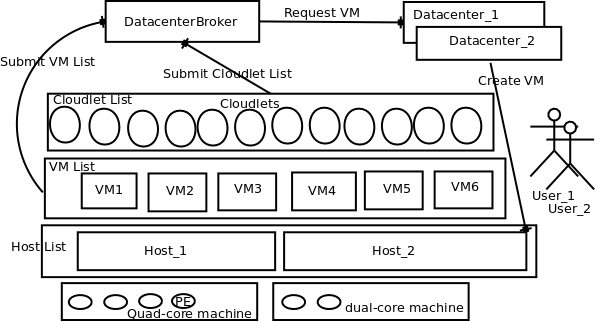
\includegraphics[width=\textwidth]{resources.png}
 }
 \caption{CloudSim scheduling operations}
 \label{fig:scheduling}
\end{figure}
Figure~\ref{fig:scheduling} depicts the overview of resource scheduling and the architecture. A list of cloudlets and a list of virtual machines are created and broker decides which cloudlet to be scheduled to execute next. Hosts are defined and each of the VMs is assigned to a host. Each cloudlet is assigned to a VM, and the Pe:s are shared among the VMs in a host and the executing cloudlets among the VMs. Complicated real-world cloud scenarios could be simulated by extending the available classes appropriately.

\SubSection{Design}
The scheduling algorithms are incorporated into CloudSim and evaluated using the available constructs of CloudSim and appropriately extending them. The method, $init()$ calls $initCommonVariable()$, which itself calls the $initialize()$ to initialize CloudSim for the simulation.
\begin{verbatimtab}
CloudSim.init(
    num_user, calendar, trace_flag);
\end{verbatimtab}
$DataCenter$ is the resource provider which simulates the infrastructure as a service. $DatacenterCharacteristics$ defines the static properties of a resource. $DataCenter$ is initialized by,
\begin{verbatimtab}
DataCenter datacenter0 = 
    createDatacenter("Datacenter0");
\end{verbatimtab}
Then the broker is created by calling,
\begin{verbatimtab}
DataCenterBroker broker = createBroker();
\end{verbatimtab}
Virtual machines are created and added to a list of virtual machines. The list is submitted to the broker. Similarly, cloudlets are created and added to a list of cloudlets. The list too is submitted to the broker. Finally the simulation is started and broker handles the allocation of VMs to the hosts and cloudlets to the VMs, while deciding which of the available cloudlets to be executed next. $CloudSimShutdown$ waits for termination of all CloudSim user entities to determine the end of simulation. An object of this class is created by CloudSim upon initialisation of the simulation.
\begin{verbatimtab}
CloudSim.init() -> 
    CloudSim.initCommonVariable()
\end{verbatimtab}
This avoids the need to manually terminate the user entities upon the end of simulation, by calling the $CloudSimShutdown()$. This object signals the end of simulation to $CloudInformationService (CIS)$ entity.
\begin{verbatimtab}
public CloudSimShutdown(String name,
    int numUser) throws Exception { .. }
\end{verbatimtab}
The total number of cloud user entity plays an important role to determine whether all hostList should be shut down or not. The hostList will be shutdown, unless one or more users are still not finished. It is important to give a correct number of total cloud user entity to avoid CloudSim hanging or displaying a weird behaviour. 

\SubSection{Implementation}
Scheduling of resources are modelled at host and VM levels in CloudSim. At the host level, fractions of the total available processing element is shared across the VMs running in the host. This is handled by the $VmScheduler$ classes. Similarly, the resources are shared among the cloudlets running in a single VM at the VM level, by the $CloudletScheduler$ classes. Classes ${X|Y}SchedulerSpaceShared$ implement the space shared system using FCFS, where ${X|Y}SchedulerTimeShared$ implement the time shared system using RR. Here, X refers to Cloudlet and Y refers to Vm, which handle the resource allocation at the VM and host level accordingly. $VmAllocationPolicy$ chooses a host and assign the given VM to it. The default behaviour is defined by $VmAllocationPolicySimple$ which picks the host with less Pe:s in use as the host for the VM. The application level scheduling - which of the cloudlets from the broker is executed next, is defined at the broker level. Figure~\ref{fig:classdiagram} depicts the classes involved in the application and resource scheduling.
\begin{figure}[ht]
 \resizebox{\columnwidth}{!}{
  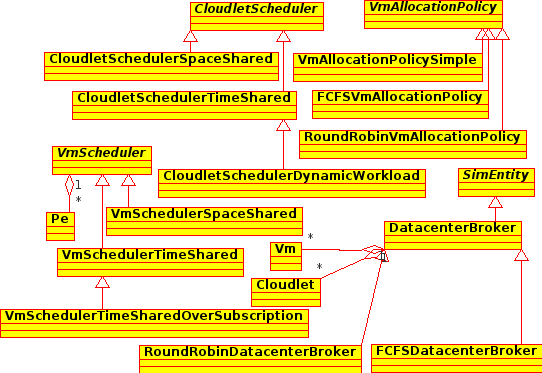
\includegraphics[width=\textwidth]{classDiagram.png}
 }
 \caption{Class Diagram depicting the core classes involved}
 \label{fig:classdiagram}
\end{figure}

The examples and default scenarios often use the TimeShared systems, which use RR algorithm. However, these policies could be mixed and the algorithm implementations for the application scheduling were tested against these different combinations of scheduling algorithms at VM and host level.

\SubSection{Scheduling Algorithms at Broker Level}
The default application scheduling is defined in $DatacenterBroker$ which picks a random cloudlet from the list of readily available cloudlets waiting to be executed next. $DatacenterBroker$ is extended and used instead, to depict the desired application scheduling algorithm.

%------------------------------------------------------------------------- 
\Section{Evaluation}
CloudSim is bundled with examples that could be extended to simulate more complicated scenarios. The existing examples and the user simulations could be executed from the folder $cloudsim-3.1-SNAPSHOT/jars$, using a command similar to the one below.
\begin{verbatimtab}
java -classpath
    cloudsim-3.1-SNAPSHOT.jar:
    cloudsim-examples-3.1-SNAPSHOT.jar 
    org.cloudbus.cloudsim.examples.
    CloudSimExample6
\end{verbatimtab}

\SubSection{Environment}
The development of experiments and the evaluation were carried on a platform of Ubuntu 12.04 LTS (precise) - 64 bit, Kernel Linux 3.2.0-56-generic and GNOME 3.4.2. The environment had 1.9 GiB memory and Intel\textregistered Core\texttrademark 2 Duo CPU T6600 @ 2.20GHz * 2 processor available. Java(TM) SE Runtime Environment was of the build 1.6.0\_31-b04.
\SubSection{Configurations}
CloudSim was configured with different configurations of jobs and resources and the experiments were conducted to study the behaviour of the scheduling algorithms. Extreme conditions for the scheduling algorithms where the program start to hang up were marked ass the upper limits and the experiments were ensured not to surpass these borders. 

Testing was carried on with 5 virtual machines and up to 4000 cloudlets having different cloudlet lengths randomly generated within the given range. Most of the initial experiments were carried ahead with the VMs having processing elements of 200, 400, 600, 800, and 1000 MIPS, 1 CPU in each virtual machines, and with 200 users.
\SubSection{Resource Allocation Algorithms}
Before evaluating the application scheduling algorithms, CloudSim was first tested with the implementations of resource allocation algorithms with the default policy of application scheduling and VM allocation to the hosts. The space shared schedulers with FCFS algorithm and the time shared schedulers with RR algorithms were tested for both the VM scheduling which is done at the host level and the cloudlet scheduling which is done at the VM level. 

The start time and the finish time of the algorithms for the same workload is plotted as figure~\ref{fig:start} and figure~\ref{fig:finish}. These plots indicate the submission time and the completion time of the cloudlets. Figure~\ref{fig:start} indicates that all the cloudlets were started almost immediately when host level scheduling was run with RR. But FCFS started the cloudlets in the order they were submitted. 
\begin{figure}[ht]
 \resizebox{\columnwidth}{!}{
  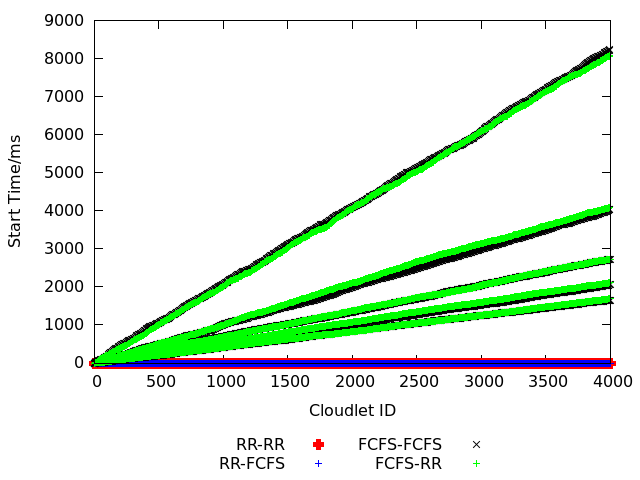
\includegraphics[width=\textwidth]{init5_4000.png}
 }
 \caption{VM and Host level Scheduling Vs Start Time}
 \label{fig:start}
\end{figure}

RR effectively shares the time window against the cloudlets. As shown by figure~\ref{fig:finish}, by switching the available time frame among the cloudlets, all the cloudlets tend to finish at the same time regardless of their starting order. However in FCFS the earlier the cloudlet starts, the earlier it finishes. This behaviour ensured a minimal minimum execution time for FCFS. However, the cloudlets that arrived later had to wait much longer even to have the Pe allocated to them. This increased the starting time or the submission time. 

In a space shared system with the FCFS algorithm, a VM is dedicated completely to a cloudlet till it finishes its execution. Hence the allocation of the VM for the respective cloudlet plays a major role in deciding the start and finish time. As virtual machines with 5 different configurations (millions of instructions per second) were used, the initial allocation of the cloudlet to the VM decides the start and finish times of the cloudlet, creating 5 different obvious straight lines of execution time. This is not observed in time shared VM level allocation, as VMs are shared across the cloudlets. The observations indicate that the VM level scheduling is dominating in submission and execution time than the host level scheduling.
\begin{figure}[ht]
 \resizebox{\columnwidth}{!}{
  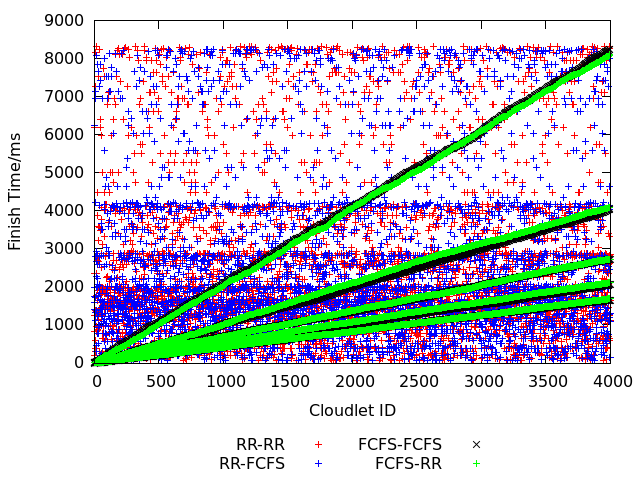
\includegraphics[width=\textwidth]{fin5_4000.png}
 }
 \caption{VM and Host level Scheduling Vs Finishing Time}
 \label{fig:finish}
\end{figure}

\SubSection{Application Scheduling Algorithms}
Mean execution time, mean submission time, mean completion time, and job scheduling success ratio of the scheduling algorithms were evaluated. Initially cloudlet scheduling with RR as well as FCFS was measured with over subscription of virtual machines to the host. Since not all the cloudlets would run concurrently, having more virtual machines with CPU higher than the total available processing elements of the host is possible and the over subscription algorithms facilitate that scenario. FCFS and RR algorithms too were evaluated at host, VM, and broker levels. Maximum resource utility algorithm has an objective function that maximizes the time frame that each of the resource is being utilized, focussing a fair resource usage avoiding over-utilization or under-utilization of a few resources. This is achieved by allocating the cloudlets to the VM with less number of Pe:s utilized. Scheduling with Maximum resource utility was also evaluated. Dynamic allocation considering the partial requirements satisfaction was evaluated as an algorithm from the utility-driven algorithms family. Mean execution time and mean submission time of these algorithms is depicted in figure~\ref{fig:met}.

\begin{figure}[ht]
 \resizebox{\columnwidth}{!}{
  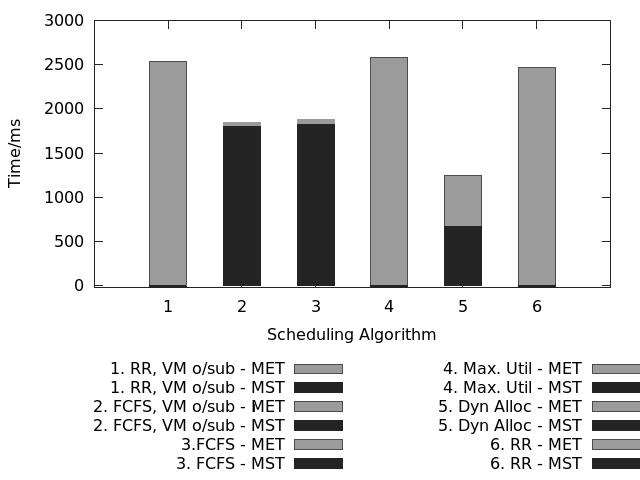
\includegraphics[width=\textwidth]{finish.png}
 }
 \caption{Mean Submission Time and Mean Execution Time of the algorithms}
 \label{fig:met}
\end{figure}

\SubSection{Observation}
As depicted by figure~\ref{fig:met}, the FCFS algorithms (both with and without the over-subscription of the VMs) perform better than RR (both with and without the over-subscription of the VMs) and Maximum resource utility algorithms, when the mean execution time is concerned. RR performs better on mean submission time, as the first slot is assigned to each of the application sooner, where the cloudlets or the tasks that are submitted later have to wait longer in FCFS, making the mean submission time higher. FCFS still performs better on mean completion time, when all the cloudlets are scheduled simultaneously.

Also the dynamic allocation outperformed all the algorithms in a hundred-fold. Partial user utility is fine tuned in this algorithm according to the tasks that are under consideration, which makes the utility-driven algorithms highly efficient for their intended target applications. Since the partial requirement satisfaction lets the user to indicate which of the requirements could be taken mildly and which ones to be taken seriously, waiting for a rare resource which is not a hard-requirement for the application is reduced. This shows that Utility-driven algorithms perform much better for the tasks that are known to the user, as the utility values could be defined accordingly such that the user utility will be maximized. 

Job scheduling success ratio remained at 100\% for all the scheduling algorithms considered. This is because the experimentation time was sufficient for all the algorithms to complete the scheduling, and there was no task that doesn't have a resource that it needs to execute. In a separate experiment involving a very limited number of resources that are of high demand by the applications showed that matchmaking algorithm scores poor in job scheduling success ration where utility-driven algorithm was still able to schedule successfully, given that the requirements could be partially satisfied.

%------------------------------------------------------------------------- 
\Section{Conclusion}
Strict matchmaking-based algorithms focus to optimize a specific objective function. User's satisfaction depends on how much his requirements are satisfied by the scheduling algorithms. User utility was proven to be reasonably high for all the criteria considered for the utility based algorithm developed considering the partial requirements satisfaction. Hence it is mandatory to develop efficient utility based scheduling algorithms to satisfy the users with heterogeneous evaluation criteria.

While criteria such as minimum execution time and minimum completion time could be a good start for evaluating the scheduling algorithms, many other parameters take higher precedence in a real cloud environment. Evaluation criteria could be developed based on the market requirements such as the cost of the cloud resource. QoS-based algorithms focus on such priorities. Developing effective evaluation criteria is essential for measuring the user satisfaction with a considerable accuracy. The effectiveness of the simulation environment to depict the real cloud scenarios is still a question to be addressed. While it is sufficient to test the prototypes and the algorithms against the simulation environment during the early phases of development, it is essential to test the production-ready algorithms against the real cloud deployments.

%------------------------------------------------------------------------- 
\Section{Future Work}
Performance of the simulation tools are far from ideal, as they try to portray a geo-distributed decentralized environment using the network and topology simulation code that is serial and manipulating the large global state that is  considered consistent. Current multi-core machines and computing clusters could be exploited by the cloud simulation tools avoiding the sequential and centralized execution of the simulations. A decentralized scheduler architecture, such as a hierarchical or a mesh-like architecture, would facilitate enhanced scalability. Nevertheless, the scalability comes with a price in efficiency. The tradeoff was estimated during the project in a conceptual manner. Further investigation would show whether a distributed scheduler architecture would be beneficial overshadowing its shortcomings in efficiency.

%------------------------------------------------------------------------- 
\Section{Acknowledgements}
Prof. Luiz Veiga provided the project idea and the motivation. Timely suggestions from Prof. Johan Montelius directed me in the right direction throughout the project. Dr. Susanna Lyne helped shaping up the project report and its presentation to its current state. My special thanks goes to these professors who helped me complete the project. As a project that is heavily used by the researchers in their research activities, CloudSim mailing list is always active with a vibrant community. I am grateful to the original developers and the community of CloudSim.

%------------------------------------------------------------------------- 
\begin{thebibliography}{1}
\bibliographystyle{acm}
\bibitem{resumo} Vasques, J. A Decentralized Utility-based Grid Scheduling Algorithm.
\bibitem{cloudsim} Calheiros, R.N., Ranjan, R., De Rose, C. A. F. and Buyya, R. CloudSim: A Novel Framework for Modeling and
 Simulation of Cloud Computing Infrastructures and Services, {\em Technical Report, GRIDS-TR-2009-1, Grid
 Computing and Distributed Systems Laboratory,} The University of Melbourne, Australia, 2009.
\bibitem{heuristics} Braun, T. D., Siegel, H. J., Beck, N., Boloni, L. L., Maheswaran, M., Reuther, A. I., and Freund, R. F. (2001). A comparison of eleven static heuristics for mapping a class of independent tasks onto heterogeneous distributed computing systems. {\em Journal of Parallel and Distributed computing, 61} (6), 810-837.
\bibitem{qosgrid} Chauhan,S.S. and Joshi, R.C. QoS Guided Heuristic Algorithms for Grid Task Scheduling. {\em International Journal of Computer Applications (0975 - 8887), Volume 2} - No.9, June 2010.
\bibitem{sufferage} Santos-Neto, E., Cirne, W., Brasileiro, F., and Lima, A. Exploiting replication and data reuse to efficiently schedule data-intensive applications on grids. In {\em Job Scheduling Strategies for Parallel Processing} (pp. 210-232). Springer Berlin Heidelberg. 2005, January.
\bibitem{emusim} Calheiros, R. N., Netto, M. A., De Rose, C. A., and Buyya, R. (2012). EMUSIM: an integrated emulation and simulation environment for modeling, evaluation, and validation of performance of cloud computing applications. {\em Software: Practice and Experience, 00-00}.
\bibitem{dcsim} Tighe, M., Keller, G., Bauer, M., and Lutfiyya, H. (2012, October). DCSim: A data centre simulation tool for evaluating dynamic virtualized resource management. In {\em Network and Service Management (CNSM), 2012 8th International Conference on} (pp. 385-392). IEEE.
\bibitem{simgrid}Casanova, H. Simgrid: A toolkit for the simulation of application scheduling. In {\em Cluster Computing and the Grid, 2001. Proceedings. First IEEE/ACM International Symposium on} (pp. 430-437). IEEE 2001.
\bibitem{oversim}Baumgart, I., Heep, B., and Krause, S. OverSim: A flexible overlay network simulation framework. In {\em IEEE Global Internet Symposium, 2007} (pp. 79-84). IEEE 2007, May.
\bibitem{peersim} Montresor, A., and Jelasity, M. PeerSim: A scalable P2P simulator. In {\em Peer-to-Peer Computing, 2009. P2P'09. IEEE Ninth International Conference on} (pp. 99-100). IEEE 2009, September.

\bibitem{cloudgridsim} Calheiros, R.N., Ranjan, R., De Rose, C. A. F. and Buyya, R. CloudSim: a toolkit for modeling and simulation of cloud computing environments and evaluation of resource provisioning algorithms. {\em Softw. Pract. Exper. 2011; 41}:23-50. Published online 24 August 2010 in Wiley Online Library (wileyonlinelibrary.com). DOI: 10.1002/spe.995
\bibitem{cloudanalyst} Wickremasinghe, B., Calheiros, R. N., and Buyya, R. (2010, April). Cloudanalyst: A cloudsim-based visual modeller for analysing cloud computing environments and applications. In {\em Advanced Information Networking and Applications (AINA), 2010 24th IEEE International Conference on} (pp. 446-452). IEEE 2010.
\bibitem{greencloud} Kliazovich, D., Bouvry, P., and Khan, S. U. (2012). GreenCloud: a packet-level simulator of energy-aware cloud computing data centers. {\em The Journal of Supercomputing, 62}(3), 1263-1283.
\bibitem{ncloudsim} Garg, S. K., and Buyya, R. (2011, December). NetworkCloudSim: modelling parallel applications in cloud simulations. In {\em Utility and Cloud Computing (UCC), 2011 Fourth IEEE International Conference on} (pp. 105-113). IEEE.
\end{thebibliography}
\end{document}

